\chapter{Background}
\label{chap:background}
In this chapter we will explore the background of the VEX system and the LLVM compiler. This chapter will show the basic design of the $\rho$-VEX processor and how the $\rho$-VEX processor operates. Further, we will also demonstrate the design of the LLVM compiler framework and how code is transformed from a high-level language such as C/C++ to a target specific assembly language.

\section{VEX System}
The $\rho$-VEX processor is based on the VEX ISA \cite{As:2008rt}. The processor uses a VLIW architecture and is designed to serve as both a application-specific processor and a general-purpose processor. During synthesis the core can be reconfigured to alter the issue-width, the amount of physical registers, the type of functional units, and other parameters.

The VEX ISA defines hardware operations as syllables. An instruction is defined as a set of multiple syllables. The VEX operations are similar to 32-bit RISC operations.

\subsection{Architecture}
The architecture of the $\rho$-VEX core is depicted in Figure \ref{fig:rvex_arch} \cite{Seedorf:2011fj}. The core uses a five-stage pipelined design. There are multiple functional units with different functionalities, such as ALU’s, multipliers, load / store units, and branch units.

\begin{figure}[ht]
\centering
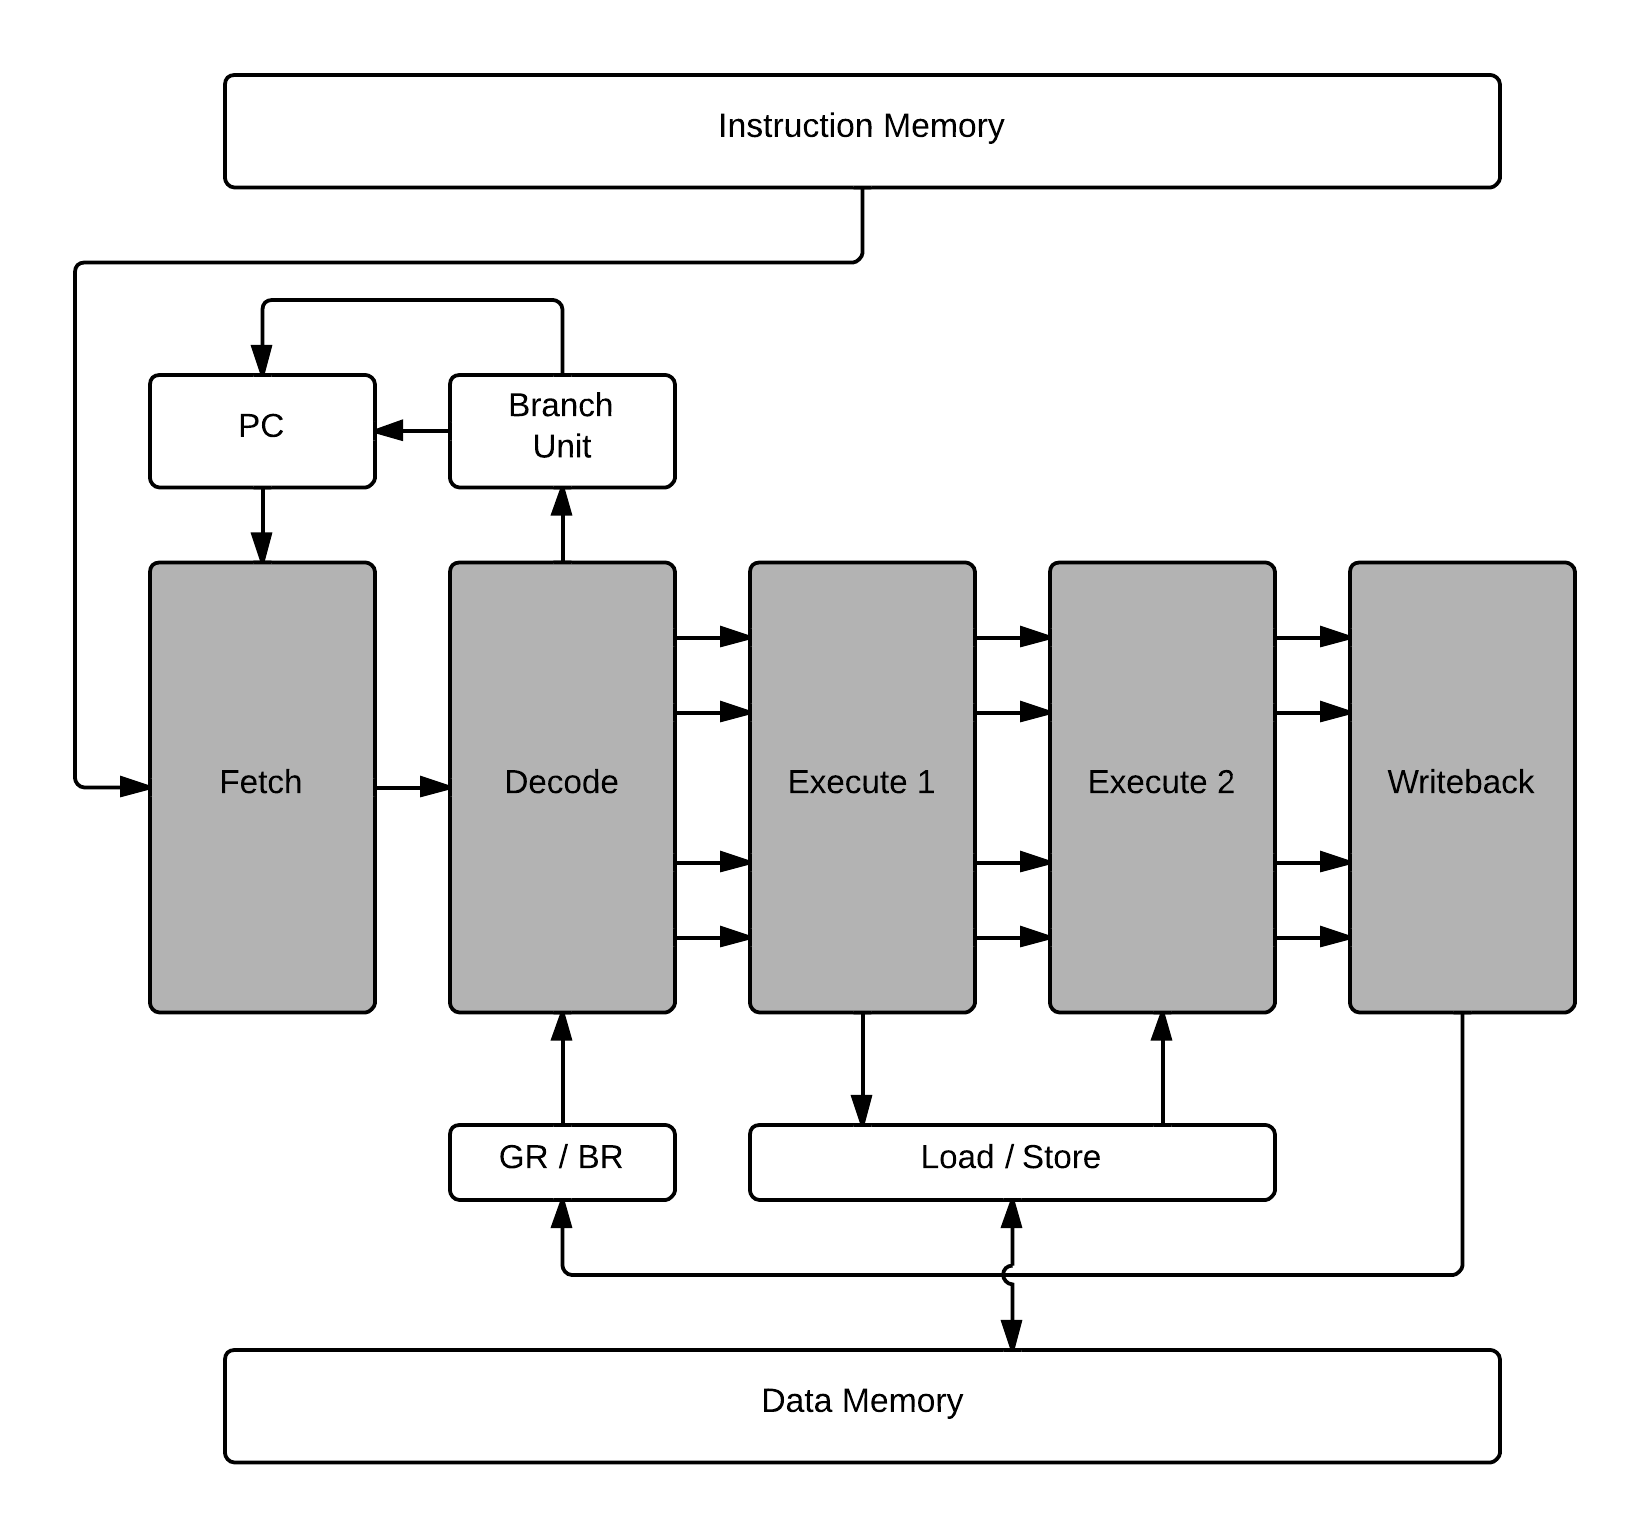
\includegraphics[width=0.8\textwidth]{2_background/img/rvex_arch.png}
\caption{$\rho$-VEX architecture \cite{Roel-Seedorf:2012qf}}
\label{fig:rvex_arch}
\end{figure}

The register file consists of 64 32-bit general-purpose registers. These registers can generally be targeted by any instruction. In addition to the general-purpose registers there also exists 8 1-bit branch registers. These registers are used by the branch operations to determine if a branch should occur.

The pipeline uses five stages to execute an instruction. For example, consider a $\rho$-VEX processor with a 4-issue organization:

\begin{itemize}
  \item \textbf{Fetch stage:} An instruction is selected from the instruction memory using the Program Counter (PC) or the Branch Target address. Note that 1 instruction contains four different operations.
  \item \textbf{Decode stage:} Each operation is decoded in parallel and the needed registers are read from the register file. 
  \item \textbf{Execute 1 stage:} In this stage, the functional units produce results for ALU operations. In addition this stage is also used to write to the data memory when Store operations are executed. The $\rho$-VEX processor uses $16*32$-bit multipliers that require two stages to produce a result. In this stage the multiplication operations are started.
  \item \textbf{Execute 2 stage:} This stage produces results for multiply operations. In addition this stage reads data from the data memory when load operations are executed.
  \item \textbf{Writeback stage:} In this stage results that have been generated in the previous stages are committed to the register file.
\end{itemize}

The $\rho$-VEX processor uses a bypass network to forward operations to other pipeline stages when needed \cite{Roel-Seedorf:2012qf}.

\subsection{ISA}
The assembly format for VEX instructions is shown in Figure \ref{fig:rvex_asm} \cite{Joseph-A.-Fisher:2012rm}. The destination of an operation is to the left of the ``='' sign, while the source operands are listed on the right-hand side. On the right-hand side both registers and immediate values can be used as source operands. The $\rho$-VEX processor does not support multiple clusters and each instruction is executed on cluster 0.

\begin{figure}[ht!]
\centering
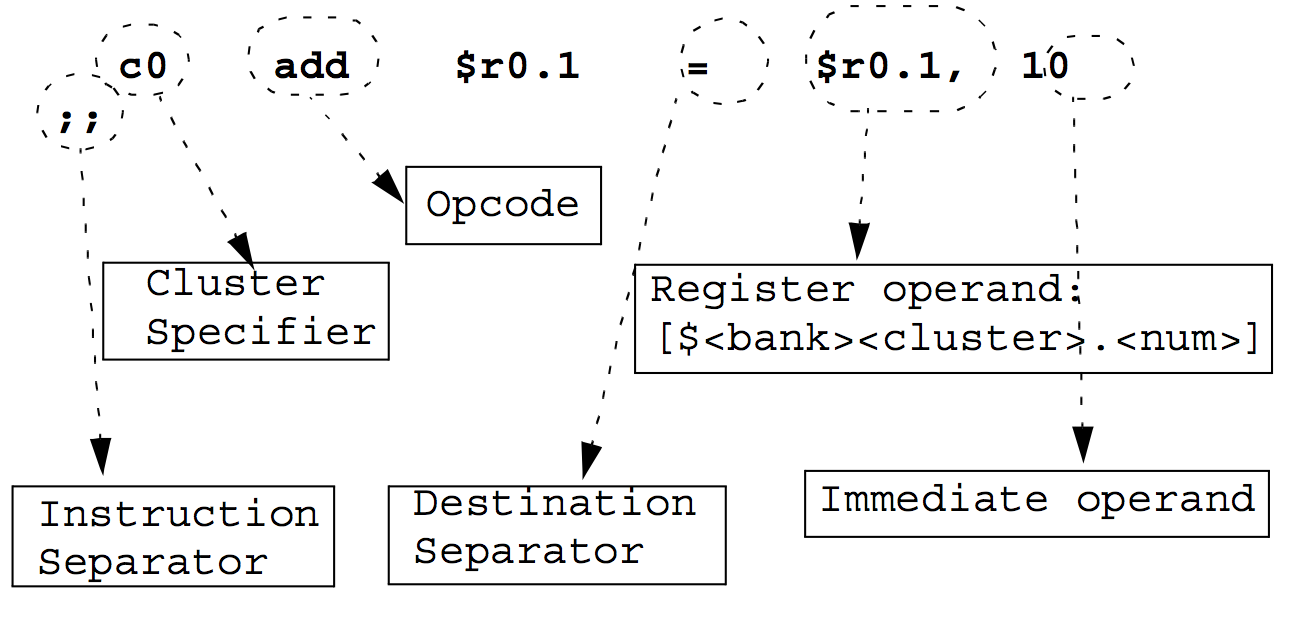
\includegraphics[width=0.8\textwidth]{2_background/img/Instructions.png}
\caption{$\rho$-VEX instruction format}
\label{fig:rvex_asm}
\end{figure}

The $\rho$-VEX processor supports 32-bit immediate values through an operations borrowing scheme. Each instruction can supports 8-bit immediate values but if larger values are required the adjacent operation is used to store the upper 24-bits of the immediate value. This means that when using large immediate value the amount of operations that can be executed decreases.

Multiple classes of $\rho$-VEX instructions exists with the following properties:

\begin{itemize}
  \item \textbf{Integer arithmetic operations:} These operations include the “traditional” RISC-style instructions such as \texttt{ADD}, \texttt{SUB}, \texttt{AND}, and \texttt{OR}. 
  \item \textbf{Multiplication operations:} The VEX ISA defines multiple multiplication operations that use the built-in $16*32$-bit multiplier. Operations include for example: Multiply Low 16 * Low 16, etc. 
  \item \textbf{Logical and Select operations:} These operations are used to compare two registers to each other or to select between two values based on the result of a branch register. Operations include: \texttt{CMPEQ}, \texttt{CMPNEQ}, etc.
  \item \textbf{Memory operations:} Operations that load and store data from the data memory. Operations exist to store and load operands of different sizes such as \texttt{LDW}, \texttt{LDH} and \texttt{LDB}.
  \item \textbf{Control operations:} These operations are used to control the Program Counter of the $\rho$-VEX processor. Operations include: \texttt{GOTO}, \texttt{CALL}, \texttt{BR}, and \texttt{RETURN}.
\end{itemize}

\subsection{Run-time architecture}
The $\rho$-VEX Run-Time architecture defines the software conventions that are used during compilation, linking and execution of $\rho$-VEX executables. $\rho$-VEX programs are executed in a 32-bit environment where integers, longs, and pointers are 32-bit values. 

The following $\rho$-VEX register classes are used:
\begin{itemize}
  \item \textbf{Scratch registers:} Caller-saved registers that are destroyed during function calls.
  \item \textbf{Preserved registers:} Callee-saved registers that must not be destroyed during procedure calls.
  \item \textbf{Constant registers:} Contains a value that cannot be changed.
  \item \textbf{Special registers:} Used during call / return operations.
\end{itemize}

The \ref{tbl:rvex_reg} described the properties of all the available $\rho$-VEX registers.

\begin{table}
  \centering
    \begin{tabular}{|l|l|p{10cm}|}
    \hline
    \textbf{Register} & \textbf{Class} & \textbf{Description}   \\ \hline
    \texttt{\$r0.0}         & Constant  & Constant register 0  \\ \hline
    \texttt{\$r0.1}         & Special   & \textbf{Stack-pointer:} Holds the limit of the current stackframe. 
                                          The SP is preserved across function calls.  \\ \hline
    \texttt{\$r0.2}         & Scratch   & \textbf{Struct return pointer:} If a function returns a struct or union the register
                                          contains the memory adres of the value being returned.  \\ \hline
    \texttt{\$r0.3-\$r0.10} & Scratch   & \textbf{Arguments and return values:} Arguments that do not fit in the registers are
                                          passed using the main memory.  \\ \hline
    \texttt{\$r0.11-\$r0.56}& Scratch   & Caller-saved scratch registers.  \\ \hline
    \texttt{\$r0.57-\$r0.63}& Preserved & Callee-saved registers that need to be preserved across function calls.  \\ \hline
    \texttt{\$l0.0}         & Special   & \textbf{Link register:} Used to store the return adres when a function call is 
                                          performed.  \\ \hline
    \texttt{\$pc0.0}        & Special   & \textbf{Program Counter}  \\ \hline
    \texttt{\$b0.0-\$b0.7}  & Scratch   & \textbf{Branch registers:} Caller-saved registers.  \\ \hline
    \end{tabular}
  \caption{$\rho$-VEX Register usage \cite{Joseph-A.-Fisher:2012rm}}
  \label{tbl:rvex_reg}
\end{table}

\section{LLVM Compiler infrastructure}
LLVM is based on the classic three-stage compiler architecture depicted in figure \ref{fig:compiler_structure}. The compiler uses a number language-specific frontends, an optimizer and target-specific backends. Each module consists of a number of generic passes that are used to transform the code. This modular design enables compiler designers to introduce new passes and parts of the compiler without having to change the existing framework. Support for a new processor can be added by building a new back-end. The existing frontend and optimizer can be reused for the new compiler.

% FIXME pas plaatje aan want in plaatje staat frontend en back-end, moet worden frontend, backend

\begin{figure}[ht]
\centering
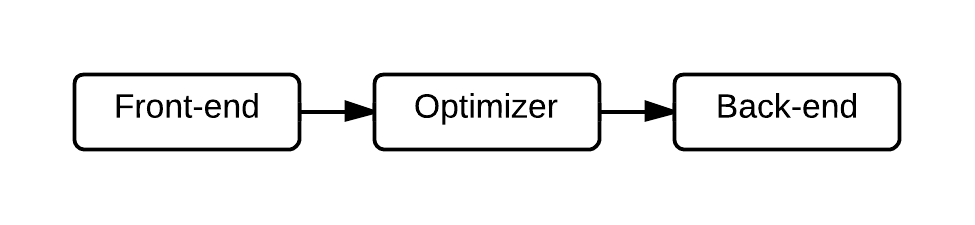
\includegraphics[width=0.8\textwidth]{2_background/img/Basic_compiler.png}
\caption{Basic compiler structure}
\label{fig:compiler_structure}
\end{figure}

The frontend is used to transform the plain text source code of a program into an intermediate representation that will be used during compilation process. This transformation is achieved by performing the following steps:

\begin{enumerate}
  \item \textbf{Lexical analysis:} Break input into individual tokens.
  \item \textbf{Syntax analysis:} Using a grammar, the sequence of tokens is transformed into a parse tree which represents the structure of the program. Clang uses a handwritten recursive descent parser for this transformation
  \item \textbf{Semantic analysis:} Semantic information is added to the parse tree, type checking is performed, and a symbol table is built.
\end{enumerate}

The resulting abstract syntax tree (AST) is transformed into LLVM IR and passed to the optimizer and backend of the compiler. These parts of the compilation process are completely language agnostic and do not require any other information from the backend.

The optimizer is used to analyze and optimize the program. Optimization such as dead code elimination and copy propagation are performed during this phase but also more advanced operations that extract ILP, such as loop vectorization \cite{llvm-loop:2014}, can be enabled.

The back-end optimizes and generates code for a specific architecture. The LLVM IR is transformed into processor specific assembly instructions. In addition the backend also allocates registers, and schedules the instructions.

\subsection{Current frontends}
% FIXME can this be merged?
The modular design of LLVM enables the compiler to be used as a part of the existing GCC compiler. For example, the dragonegg GCC plugin \cite{dragonegg:2014} is designed to replace the GCC code generator and optimizer with the LLVM backend. This would enable LLVM to be able to use the existing GCC based frontends and supported languages.

Clang has been developed to allow LLVM to operate independently of GCC. Clang is a frontend supporting C, C++, and ObjC. The frontend is designed to be closely integrated with the Integrated Development Environment (IDE) allowing more expressive diagnostic messages. In addition, Clang also aims to provide faster compilation and lower memory usage \cite{clang:features}.

\subsection{LLVM IR}
The frontend transforms a source code into the LLVM Intermediate representation (LLVM IR). The LLVM IR is used to represent a high level language cleanly in a target independent way and is used during all phases of compilation. Instructions are similar to RISC instructions and can use three operands. Control flow instructions and type specific load/store instructions are used and an infinite amount of registers are available in Single Static Assignment (SSA) form. The LLVM IR is available in three different forms: human readable text, binary form, and an in-memory form \cite{llvm:presentation}.

The LLVM IR is designed to expose high-level information for further optimization. Examples of high-level information include dataflow analysis using the SSA form, control-flow graphs, language independent type information and explicit use of pointer arithmetic. 

Primitives such as voids, floats and integers are natively supported in the LLVM IR. The bit width of the integers can be defined manually. Pointers, arrays, structures and functions are derived from these basic types. The operations that are supported in LLVM IR are contained in the Instruction Selection DAG (ISD) namespace.

Object-oriented constructs such as classes and virtual methods are not natively supported but can be built using the existing type system. For example, a C++ class can be represented by a struct and a list of methods. 

The SSA-based dataflow form allows the compiler to efficiently perform code optimizations such as dead code elimination and constant propagation. 

Figure \ref{lst:C_Example} depicts an example program in C. The equivalent LLVM IR representation is depicted in figure \ref{lst:LLVM_IR}.

\lstset{numbers=none, captionpos=b}
\begin{lstlisting}[language=C,caption={C example program},label=lst:C_Example]
int main() {
  int sum = 1;

  while(sum < 10)
  {
    sum = sum + 1;
  }
  return sum;
}
\end{lstlisting}


\lstset{numbers=none, captionpos=b}
\begin{lstlisting}[language=llvm,caption={LLVM Intermediate representation},label=lst:LLVM_IR]

define i32 @main() nounwind ssp uwtable {
  %1 = alloca i32, align 4
  %sum = alloca i32, align 4
  store i32 0, i32* %1
  store i32 1, i32* %sum, align 4
  br label %2

; <label>:2                                       ; preds = %5, %0
  %3 = load i32* %sum, align 4
  %4 = icmp slt i32 %3, 10
  br i1 %4, label %5, label %8

; <label>:5                                       ; preds = %2
  %6 = load i32* %sum, align 4
  %7 = add nsw i32 %6, 1
  store i32 %7, i32* %sum, align 4
  br label %2

; <label>:8                                       ; preds = %2
  %9 = load i32* %sum, align 4
  ret i32 %9
}

\end{lstlisting}

\subsection{Code generation}
During code generation the optimized LLVM IR is translated into machine-specific assembly instructions. The modular design of LLVM enables generic algorithms to be used for this process. 

A backend is described in a domain-specific language (DSL) called \texttt{tablegen}. The \texttt{tablegen} files describe properties of a backend such as available instructions, registers, calling convention and pipeline structure. During compilation of LLVM the \texttt{tablegen} files are converted into a C++ description of the backend. \texttt{tablegen} has been specifically designed to describe the backend structure in a flexible and generic way. Common features can be more easily described using \texttt{tablegen}. For example the \texttt{add} and \texttt{sub} instruction are almost identical and using \texttt{tablegen} can be described in a more generic way. This results in less repetition and reduces the chance of error in the backend description.

Because of the generic description of the backend large amount of code can be reused by each backend. Algorithms such as register allocation and instruction selection operate on the generic \texttt{tablegen} descriptions and do not require target specific hooks to operate correctly. An additional advantage of this approach is that multiple algorithms are available to achieve certain functionality. For example, LLVM offers the developer a choice between four different register allocation algorithms. Each algorithm has a number of advantages and disadvantages and the developer can choose between an algorithm which matches the target processor best.

At the moment not all parts of the backend can be described in \texttt{tablegen} and hand written C++ code is still needed. As LLVM matures more parts of the backend description should be integrated into the backend. 

Figure \ref{fig:codegen_process} shows the basic code generation process. Each block can consist of multiple LLVM passes. For example the instruction selection phase consists of multiple passes that transform the input LLVM IR into a DAG that only contains instructions and types that are supported by the target processor.
\begin{figure}[ht]
\centering
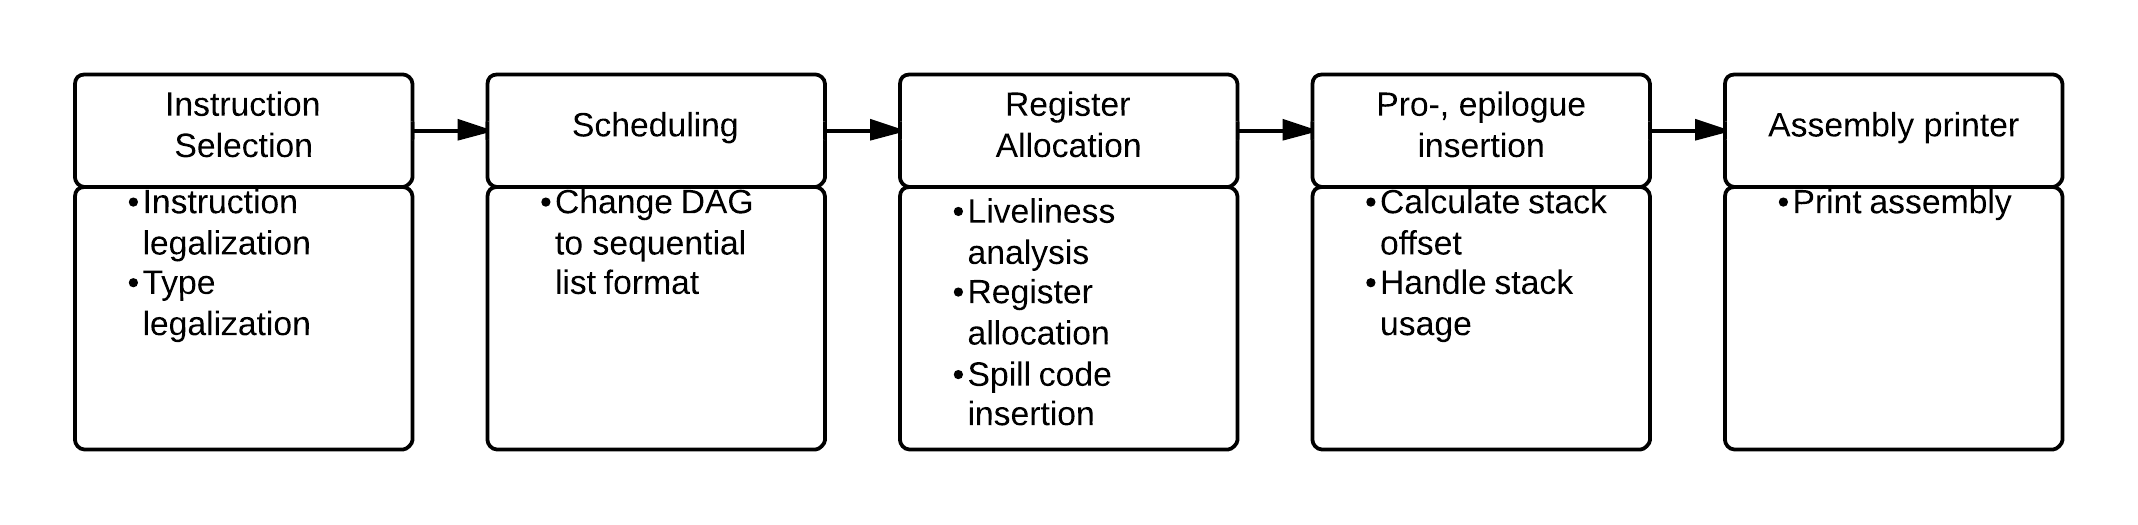
\includegraphics[width=0.8\textwidth]{2_background/img/Codegen.png}
\caption{Basic codegeneration process}
\label{fig:codegen_process}
\end{figure}

\subsection{Scheduling} % (fold)
\label{sub:scheduling}
The LLVM compiler uses basic blocks to schedule instructions. A basic block is a block of code that has exactly one entry point and one exit point. This means that no jump instruction exists with a destination in the block. 

LLVM uses the \texttt{MachineBasicBlock} (MBB) class to represent a Basic Block. A MBB contains a list of \texttt{MachineInstr} instances. The \texttt{MachineInstr} class is an abstract way to represent instructions for the target processor.

Multiple MBB are used to create a \texttt{MachineFunction} instance. The \texttt{MachineFunction} class is used to represent a LLVM IR function. In addition to a list of MBB the MachineFunction also contains references to the \texttt{MachineConstantPool}, \texttt{MachineFrameInfo}, \texttt{MachineFunctionInfo}, and \texttt{MachineRegisterInfo}. These classes keep track of target specific function information such as which constants are spilled to memory, the objects that are allocated on the stack, target specific function information, and which registers are used. 

% subsection scheduling (end)

\subsection{Current backends}
The current version of the LLVM compiler supports the following processor architectures:

\begin{itemize}
  \item \textbf{ARM:} RISC type processor designed for use in embedded systems.
  \item \textbf{AArch64:} Targets ARMv8 ISA that has support for 64-bit architectures.
  \item \textbf{Hexagon:} 32-bit DSP processor developed by Qualcomm. Targets a VLIW type processor
  \item \textbf{MIPS:} One of the original RISC type processors \cite{Hennessy:1983:DHP:892745}.  
  \item \textbf{MBlaze:} Derivative of the MIPS processor developed by Xilinx for use in FPGAs.
  \item \textbf{MSP430:} 16-bit processor developed by Texas Instruments.
  \item \textbf{NVPTX:} CUDA backend targeting NVIDIA GPUs.
  \item \textbf{PowerPC:} RISC type processor developed by IBM.
  \item \textbf{R600:} Backend that targets R600 AMD GPUs.
  \item \textbf{Sparc:} One of the original RISC type processors \cite{4874}.
  \item \textbf{SystemZ:} Processor used in IBM Mainframes.
  \item \textbf{X86:} General purpose processor.
  \item \textbf{XCore:} 32-bit RISC type processor.
\end{itemize}

Backends that target other architectures also exist but these are not included in the distribution of the LLVM compiler and are not actively maintained by the LLVM community. The Hexagon, NVPTX, and R600 backends are of special interest because these backends target VLIW processors or massive parallel systems such as GPUs. The Hexagon processor demonstrates that it is possible to build a LLVM backend that targets a general purpose VLIW type processor.

\section{Verification}
Verification of the LLVM compiler is extremely important. Performance of the generated binaries is irrelevant if only half of the binaries produce a correct result. The LLVM compiler will be verified by simulating the generated binaries. 

Two simulators are available: XSTsim and Modelsim. XSTsim is an ISA simulator that can simulate a 4-issue $\rho$-VEX processor. Output of the simulator is customizable and the simulator is fast enough to simulate large executables. Modelsim is used to perform a complete functional simulation of the $\rho$-VEX processor. The Modelsim simulation provides the highest accuracy because the hardware description files of the $\rho$-VEX processor are used during simulation. The disadvantage of using Modelsim is the performance. Simulation of an executable will take a long time because the complete processor is simulated.

Writing test programs that generate certain instruction sequences will be used to verify the compiler. The output of these test programs will be compared to the expected result to check for errors in the backend.

Writing test programs that have a high coverage of all the possible output patterns is impossible. To further verify the compiler we will compile benchmark programs that simulate certain. The output of the benchmarking programs will be compared to expected outputs to check for errors in the compiler.

\section{Conclusion}
This chapter presented the basic design of the $\rho$-VEX processor and of the LLVM compiler framework. The $\rho$-VEX processor is a VLIW-type processor that uses RISC like instructions to operate. We presented the basic design of the processor, the instructions that are supported, register properties, and the run-time architecture has been discussed. This information will be used during implementation of the LLVM-based compiler.

We also discussed the basic working of the LLVM compiler framework. Building a $\rho$-VEX backend for the LLVM compiler is feasible because the current version of the LLVM compiler already targets a VLIW processor. 

Finally, we discussed how the LLVM compiler will be verified. The verification step is extremely important to determine whether the binaries that are generated work correctly.

\acresetall

